% Options for packages loaded elsewhere
\PassOptionsToPackage{unicode}{hyperref}
\PassOptionsToPackage{hyphens}{url}
%
\documentclass[
  11pt,
]{article}
\usepackage{amsmath,amssymb}
\usepackage{iftex}
\ifPDFTeX
  \usepackage[T1]{fontenc}
  \usepackage[utf8]{inputenc}
  \usepackage{textcomp} % provide euro and other symbols
\else % if luatex or xetex
  \usepackage{unicode-math} % this also loads fontspec
  \defaultfontfeatures{Scale=MatchLowercase}
  \defaultfontfeatures[\rmfamily]{Ligatures=TeX,Scale=1}
\fi
\usepackage[]{mathpazo}
\ifPDFTeX\else
  % xetex/luatex font selection
\fi
% Use upquote if available, for straight quotes in verbatim environments
\IfFileExists{upquote.sty}{\usepackage{upquote}}{}
\IfFileExists{microtype.sty}{% use microtype if available
  \usepackage[]{microtype}
  \UseMicrotypeSet[protrusion]{basicmath} % disable protrusion for tt fonts
}{}
\makeatletter
\@ifundefined{KOMAClassName}{% if non-KOMA class
  \IfFileExists{parskip.sty}{%
    \usepackage{parskip}
  }{% else
    \setlength{\parindent}{0pt}
    \setlength{\parskip}{6pt plus 2pt minus 1pt}}
}{% if KOMA class
  \KOMAoptions{parskip=half}}
\makeatother
\usepackage{xcolor}
\usepackage[margin = 1in]{geometry}
\usepackage{longtable,booktabs,array}
\usepackage{calc} % for calculating minipage widths
% Correct order of tables after \paragraph or \subparagraph
\usepackage{etoolbox}
\makeatletter
\patchcmd\longtable{\par}{\if@noskipsec\mbox{}\fi\par}{}{}
\makeatother
% Allow footnotes in longtable head/foot
\IfFileExists{footnotehyper.sty}{\usepackage{footnotehyper}}{\usepackage{footnote}}
\makesavenoteenv{longtable}
\usepackage{graphicx}
\makeatletter
\def\maxwidth{\ifdim\Gin@nat@width>\linewidth\linewidth\else\Gin@nat@width\fi}
\def\maxheight{\ifdim\Gin@nat@height>\textheight\textheight\else\Gin@nat@height\fi}
\makeatother
% Scale images if necessary, so that they will not overflow the page
% margins by default, and it is still possible to overwrite the defaults
% using explicit options in \includegraphics[width, height, ...]{}
\setkeys{Gin}{width=\maxwidth,height=\maxheight,keepaspectratio}
% Set default figure placement to htbp
\makeatletter
\def\fps@figure{htbp}
\makeatother
\setlength{\emergencystretch}{3em} % prevent overfull lines
\providecommand{\tightlist}{%
  \setlength{\itemsep}{0pt}\setlength{\parskip}{0pt}}
\setcounter{secnumdepth}{5}
\newlength{\cslhangindent}
\setlength{\cslhangindent}{1.5em}
\newlength{\csllabelwidth}
\setlength{\csllabelwidth}{3em}
\newlength{\cslentryspacingunit} % times entry-spacing
\setlength{\cslentryspacingunit}{\parskip}
\newenvironment{CSLReferences}[2] % #1 hanging-ident, #2 entry spacing
 {% don't indent paragraphs
  \setlength{\parindent}{0pt}
  % turn on hanging indent if param 1 is 1
  \ifodd #1
  \let\oldpar\par
  \def\par{\hangindent=\cslhangindent\oldpar}
  \fi
  % set entry spacing
  \setlength{\parskip}{#2\cslentryspacingunit}
 }%
 {}
\usepackage{calc}
\newcommand{\CSLBlock}[1]{#1\hfill\break}
\newcommand{\CSLLeftMargin}[1]{\parbox[t]{\csllabelwidth}{#1}}
\newcommand{\CSLRightInline}[1]{\parbox[t]{\linewidth - \csllabelwidth}{#1}\break}
\newcommand{\CSLIndent}[1]{\hspace{\cslhangindent}#1}
\usepackage{setspace}\doublespacing
\usepackage[left]{lineno}
\nolinenumbers
\usepackage{dcolumn}
\usepackage{caption}
\usepackage{afterpage}
\usepackage{siunitx}
\usepackage{amsmath}
\ifLuaTeX
  \usepackage{selnolig}  % disable illegal ligatures
\fi
\IfFileExists{bookmark.sty}{\usepackage{bookmark}}{\usepackage{hyperref}}
\IfFileExists{xurl.sty}{\usepackage{xurl}}{} % add URL line breaks if available
\urlstyle{same}
\hypersetup{
  pdftitle={Controls for non-independence should reflect the data-generating process},
  pdfauthor={Scott Claessens; Thanos Kyritsis; Quentin D Atkinson},
  hidelinks,
  pdfcreator={LaTeX via pandoc}}

\title{Controls for non-independence should reflect the data-generating process}
\author{Scott Claessens\footnote{School of Psychology, University of Auckland; School of Psychology, University of Kent; \href{mailto:scott.claessens@gmail.com}{\nolinkurl{scott.claessens@gmail.com}}} \and Thanos Kyritsis\footnote{School of Psychology, University of Auckland} \and Quentin D Atkinson\footnote{School of Psychology, University of Auckland}}
\date{January 16, 2025}

\begin{document}
\maketitle

\linenumbers

In our article\textsuperscript{1}, we simulated national-level trait data with
non-independence due to spatial diffusion or shared language ancestry. These are
plausible scenarios from which we can evaluate the ability of different methods
to recover the ``true'' cross-national correlation. We used these simulations to
evaluate the performance of widely-used statistical controls for
non-independence and showed that these methods do not result in a satisfactory
reduction in false positives. This finding holds and is concerning regardless of
our ability to identify an alternative class of models that performs better. We
then further showed that Bayesian random effects models incorporating explicit
assumptions about the data-generating process do indeed perform much better. In
particular, the Bayesian model controlling for spatial proximity was most
effective at reducing false positives in spatially non-independent data, and the
Bayesian model controlling for linguistic proximity was most effective at
reducing false positives in ``language tree'' non-independent data.

In their Matters Arising, Wolfer and Koplenig\textsuperscript{2} (henceforth W\&K) seem
to imply that we conclude from this simulation that models controlling for
spatial and linguistic proximity should \emph{always} outperform alternatives and
should therefore \emph{always} be the models of choice when analysing autocorrelated
cross-national data. To rebut this claim, W\&K simulate cross-national data with
another form of non-independence: autocorrelation due to shared religious
ancestry. From these simulation results, W\&K argue that models controlling for
spatial and linguistic proximity are no more effective at reducing false
positives compared to models with alternative controls. W\&K conclude that our
original simulation results were due purely to a methodological artefact that
they label ``data leakage'', where the same covariance matrix is used to generate
and analyse the data.

To be clear, we never claimed that models controlling for spatial and linguistic
proximity should always be the model of choice when analysing cross-national
data. In fact, we explicitly caution against this in our article: ``we did not
simulate other sources of non-independence that potentially exist in real
cross-national datasets\ldots{} additional controls will be required to ensure that
these sources of non-independence do not confound cross-national
inferences''\textsuperscript{1} (p.~8).

We expand on this point here. Instead of being used as a one-size-fits-all
recipe, controls for non-independence should reflect the data-generating process
for the particular dataset at hand. As we would expect, if you simulate data
with one source of non-independence and run regressions controlling for a
different source of non-independence, the performance will be affected. In our
own simulations, for example, we already showed that controls for spatial
proximity did not necessarily deal with linguistic non-independence, and
controls for linguistic proximity did not necessarily deal with spatial
non-independence.

The same is true for the simulations from W\&K. While we agree that there is a
relationship between linguistic and religious traits, the covariation implied by
these two forms of cultural ancestry are different, resulting in only a moderate
correlation between linguistic and religious proximities in nations around the
world (\emph{r} =
0.38)
and an even weaker correlation between spatial and religious proximities (\emph{r} =
0.20).
Given these differences, it is no surprise that models controlling for spatial
and linguistic proximity do not eliminate false positives when dealing with
autocorrelation due to religious ancestry. Space and language are poor proxy
controls for religion.

It is interesting though that the costs of getting this wrong are not huge.
While models controlling for spatial and linguistic proximity fail to
completely eliminate false positives in the religious-autocorrelation
simulations from W\&K, they still arguably perform just as well, if not better,
compared to the original models we tested. For example, the Bayesian models
controlling for linguistic proximity are the only models that are able to
eliminate false positives when there is weak autocorrelation on the predictor
variable (the red line in W\&K's Figure 1).

We thank W\&K for highlighting that we used the same matrices for generating and
analysing data in our simulations. While we assumed this was obvious, in
hindsight, we could have gone to greater lengths to emphasise this feature of
our analysis to readers. However, we do not think ``data leakage'' is the right
label for this. This label is often used in the context of machine learning and
other predictive modelling, where information from a training dataset is
unintentionally incorporated into a test dataset that the model is later used to
predict\textsuperscript{3}. There was no such unintentional ``leakage'' in our article.
We used simulated data to evaluate the performance of different causal inference
models, including versions of the actual data-generating model, against a known
ground truth. This is a standard design feature of simulation-based model
validation in the causal inference literature\textsuperscript{4,5} and not
``leakage''.

The broader lesson here is that researchers need to deal with non-independence
in their national-level datasets, and when we do, our decisions must be informed
by our causal understanding of the processes at work, not the application of a
one-size-fits-all recipe. W\&K are right to note that the data-generating process
is often uncertain to researchers, especially with observational national-level
data. But the fact that we may not be able to precisely specify this process
does not justify resorting to simpler methods that we know do not capture the
process.

There are several ways that researchers can deal with their uncertainty about
the true data-generating process. First, researchers can try including multiple
matrices in the analysis, as we did in our simulations, with little or no cost
in false positives or loss of power. Since the random effects models scale the
relative importance of different matrices according to the amount of ``signal'' in
the data, it often does not hurt to include multiple matrices in the analysis,
provided that these are motivated by a plausible model of the data-generating
process.

Second, researchers can integrate over their uncertainty in the data-generating
process. For example, cultural phylogenetic analyses often average over
uncertainty in the language ancestry that is thought to have created
autocorrelation in the data, iterating the model over many samples from a
posterior set of language phylogenies\textsuperscript{6,7}.

\begin{figure}
\centering
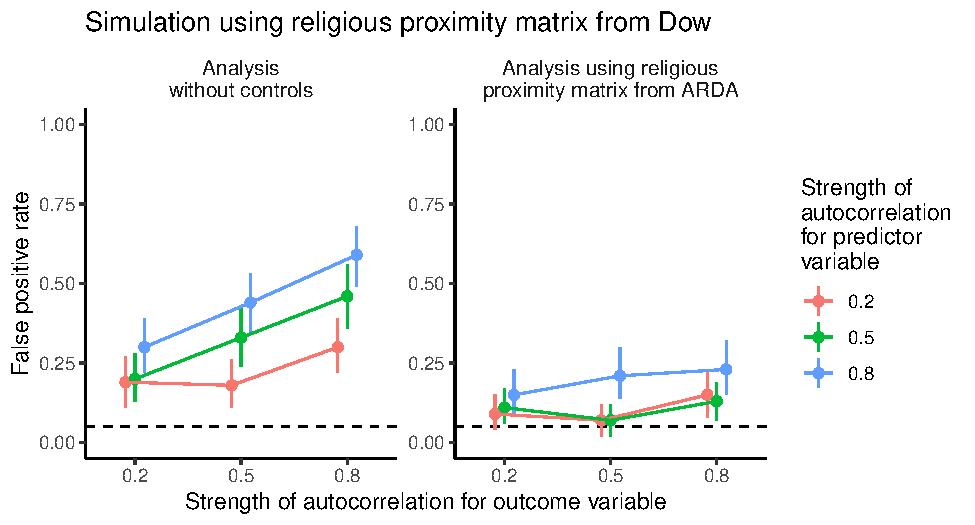
\includegraphics{manuscript_files/figure-latex/plot-1.pdf}
\caption{\label{fig:plot}Results from additional simulations using an alternative religious proximity matrix to analyse the data. False positive rates were operationalised as the proportion of models that estimated a slope with a 95\% credible interval excluding zero. Points represent raw proportions of false positives out of 100 models, ranges represent 95\% bootstrap confidence intervals (n = 1000 bootstrap samples), and dashed lines indicate the 5\% false positive rate that is expected due to chance. Colours indicate whether the strength of autocorrelation for the predictor variable is 0.2 (red), 0.5, (green) or 0.8 (blue). ARDA = Association of Religion Data Archives.}
\end{figure}

Third, researchers can use an approximation of the data-generating process. In
the case of religious ancestry, for example, our simulation results still stand
when we use \emph{different} matrices to generate and analyse the data, so long as
those matrices approximate the same underlying process (i.e., not a different
process like linguistic ancestry). To show this, we repeat the simulations from
W\&K but use an alternative religious proximity matrix to analyse the simulated
datasets. This alternative religious proximity matrix was created using data
from the Association of Religion Data Archives\textsuperscript{8,9} (see
Supplementary Information). The matrix has higher resolution than W\&K's matrix
and is more strongly correlated with W\&K's matrix (\emph{r} =
0.81)
than language or geography. Our simulations with this alternative matrix show
that valid approximations of the true data-generating process can effectively
reduce false positive rates, even when the covariance matrices used to generate
and analyse the data are not identical (Figure \ref{fig:plot}).

As a final point, while we agree that these Bayesian random effects models can
take a long time to run when iterated across hundreds of simulated datasets, we
note that, contrary to the claims from W\&K, \emph{individual} models in our
simulation took no longer than a minute to sample on a standard laptop.

\nolinenumbers

\subsection*{Data availability}

Data on geographic, linguistic, and religious proximity can be found on
GitHub: \url{https://github.com/ScottClaessens/crossNationalSimulations}

\subsection*{Code availability}

The code necessary to reproduce our simulations and generate the manuscript can
be found on GitHub: \url{https://github.com/ScottClaessens/crossNationalSimulations}

\subsection*{Competing interests}

The authors declare no competing interests.

\hypertarget{references}{%
\section*{References}\label{references}}
\addcontentsline{toc}{section}{References}

\hypertarget{refs}{}
\begin{CSLReferences}{0}{0}
\leavevmode\vadjust pre{\hypertarget{ref-Claessens2023}{}}%
\CSLLeftMargin{1. }%
\CSLRightInline{Claessens, S., Kyritsis, T. \& Atkinson, Q. D. \href{https://doi.org/10.1038/s41467-023-41486-1}{Cross-national analyses require additional controls to account for the non-independence of nations}. \emph{Nature Communications} \textbf{14}, 5776 (2023).}

\leavevmode\vadjust pre{\hypertarget{ref-Wolfer2024}{}}%
\CSLLeftMargin{2. }%
\CSLRightInline{Wolfer, S. \& Koplenig, A. Leakage explains the apparent superiority of {Bayesian} random effect models - a preregistered comment on {Claessens, Kyritsis and Atkinson (2023)}. (2024) doi:\href{https://doi.org/10.31219/osf.io/ex267}{10.31219/osf.io/ex267}.}

\leavevmode\vadjust pre{\hypertarget{ref-Kaufman2012}{}}%
\CSLLeftMargin{3. }%
\CSLRightInline{Kaufman, S., Rosset, S., Perlich, C. \& Stitelman, O. \href{https://doi.org/10.1145/2382577.2382579}{Leakage in data mining: Formulation, detection, and avoidance}. \emph{ACM Transactions on Knowledge Discovery from Data} \textbf{6}, 1--21 (2012).}

\leavevmode\vadjust pre{\hypertarget{ref-Pearl2000}{}}%
\CSLLeftMargin{4. }%
\CSLRightInline{Pearl, J. \emph{Causality: Models, Reasoning and Inference}. (Cambridge University Press, Cambridge, UK, 2000).}

\leavevmode\vadjust pre{\hypertarget{ref-McElreath2020}{}}%
\CSLLeftMargin{5. }%
\CSLRightInline{McElreath, R. \emph{Statistical Rethinking: A {B}ayesian Course with Examples in {R} and {Stan}}. (CRC Press, 2020).}

\leavevmode\vadjust pre{\hypertarget{ref-Sheehan2023}{}}%
\CSLLeftMargin{6. }%
\CSLRightInline{Sheehan, O. \emph{et al.} \href{https://doi.org/10.1038/s41562-022-01471-y}{Coevolution of religious and political authority in {Austronesian} societies}. \emph{Nature Human Behaviour} \textbf{7}, 38--45 (2023).}

\leavevmode\vadjust pre{\hypertarget{ref-Watts2016}{}}%
\CSLLeftMargin{7. }%
\CSLRightInline{Watts, J., Sheehan, O., Atkinson, Q. D., Bulbulia, J. \& Gray, R. D. \href{https://doi.org/10.1038/nature17159}{Ritual human sacrifice promoted and sustained the evolution of stratified societies}. \emph{Nature} \textbf{532}, 228--231 (2016).}

\leavevmode\vadjust pre{\hypertarget{ref-Brown2018}{}}%
\CSLLeftMargin{8. }%
\CSLRightInline{Brown, D., Mataic, D. R., Bader, C. \& Finke, R. \href{https://www.thearda.com/}{{The Association of Religion Data Archives: ARDA}}. (2018).}

\leavevmode\vadjust pre{\hypertarget{ref-Kyritsis2022}{}}%
\CSLLeftMargin{9. }%
\CSLRightInline{Kyritsis, T., Matthews, L. J., Welch, D. \& Atkinson, Q. D. \href{https://doi.org/10.1017/ehs.2022.40}{Shared cultural ancestry predicts the global diffusion of democracy}. \emph{Evolutionary Human Sciences} \textbf{4}, e42 (2022).}

\end{CSLReferences}

\newpage

\section*{Supplementary Information}

\subsection*{Data-generating model for simulations}

Following the approach in our initial article (Claessens et al., 2023), we 
simulated data for 150 nations $i$ with varying degrees of religious 
autocorrelation for outcome $y$ and predictor $x$ using the following
generative model:

\begin{align}
\begin{bmatrix}y_i\\x_i \end{bmatrix} &\sim \text{MVNormal}
\begin{pmatrix}\begin{bmatrix}\alpha_y\\\alpha_x \end{bmatrix},
\textbf{S}\end{pmatrix} \nonumber \\
\alpha_y &\sim \text{Normal}(0, \sqrt{\lambda} \cdot \Sigma_\text{Dow}) 
\nonumber \\
\alpha_x &\sim \text{Normal}(0, \sqrt{\rho} \cdot \Sigma_\text{Dow}) 
\nonumber \\
\textbf{S} &= 
\begin{pmatrix}\sqrt{1 - \lambda} & 0 \\ 0 & \sqrt{1 - \rho} \end{pmatrix}
\begin{pmatrix}1 & r \\ r & 1\end{pmatrix}
\begin{pmatrix}\sqrt{1 - \lambda} & 0 \\ 0 & \sqrt{1 - \rho} \end{pmatrix} 
\nonumber
\end{align}

In this generative model, $\Sigma_\text{Dow}$ is the national-level religious
proximity matrix that Wolfer and Koplenig (2024) constructed using data from Dow
and Karunaratna (2006). In addition, $\lambda$ and $\rho$ are autocorrelation 
parameters that represent the expected religious "signal" for outcome and 
predictor variables, respectively, and $r$ is the true cross-national 
correlation between the variables after accounting for religious
autocorrelation. We set $\lambda$ and $\rho$ to 0.2 (weak), 0.5 (moderate), or 
0.8 (strong). For simplicity, we always set $r = 0$ in this simulation. For each
parameter combination, we simulated 100 datasets, resulting in 900 datasets.

\subsection*{Analysis without controls}

We first analysed the simulated data without any control variables. The
statistical model is as follows:

\begin{align}
y_i &\sim \text{Normal}(\mu_i, \sigma) \nonumber \\
\mu_i &= \alpha + \beta x_i \nonumber \\
\alpha &\sim \text{Normal}(0, 0.5) \nonumber \\
\beta &\sim \text{Normal}(0, 0.5) \nonumber \\
\sigma &\sim \text{Exponential}(5) \nonumber
\end{align}

We fitted each model using the \textit{brms} package (Bürkner, 2017) with four 
chains, 1000 warmup samples, and 1000 post-warmup samples. We calculated the 
false positive rate as the proportion of $\beta$ slopes with 95\% credible 
intervals excluding zero.

\subsection*{Analysis using alternative religious proximity matrix}

For our next analysis, we used a religious proximity matrix of countries from 
Kyritsis et al. (2022). This matrix is based on national-level data on religious
adherence from the Association of Religion Data Archives (ARDA) together with a
family tree representing genealogical relationships between 28 religious
lineages, informed by historical sources. Since there is evidence for horizontal
transmission between some lineages, eight different cladograms were considered,
representing alternative paths of inheritance between lineages. For further
details on the construction of these religious family trees, see Kyritsis et al.
(2022).

For each of the eight cladograms, a pairwise distance matrix was generated based
on patristic distances between religious traditions. These distances were then 
converted to proximities and weighted by adherent percentages from ARDA 
using the following formula (Eff, 2008):

\[R_{rk} = \sum_{r} \sum_{k} p_{ik} p_{jr} s_{ij}\]

where $R_{rk}$ is the religious connection between countries $r$ and $k$,
$p_{ik}$ is the percentage of the population in country $k$ adhering to religion
$i$, $p_{jr}$ is the percentage of the population in country $r$ adhering to 
religion $j$, and $s_{ij}$ is the religious proximity measure between religions
$i$ and $j$. The resulting eight matrices were averaged to produce the final
matrix, which we label $\Sigma_\text{ARDA}$.

We then included this $\Sigma_\text{ARDA}$ matrix in the statistical model 
above, allowing nation random effects to covary according to alternative
religious proximities. The statistical model is as follows:

\begin{align}
y_{i} &\sim \text{Normal}(\mu_{i},\sigma) \nonumber \\
\mu_{i} &= \alpha + z_{\text{NATION}[i]}\sigma_{\alpha}\Sigma_\text{ARDA} + 
\beta x_{i} \nonumber \\
\alpha &\sim \text{Normal}(0, 0.5) \nonumber \\
\beta &\sim \text{Normal}(0, 0.5) \nonumber \\
z_{j} &\sim \text{Normal}(0, 1) \nonumber \\
\sigma_{\alpha} &\sim \text{Exponential}(5) \nonumber \\
\sigma &\sim \text{Exponential}(5) \nonumber
\end{align}

We fitted each model using the \textit{brms} package (Bürkner, 2017) with four 
chains, 1000 warmup samples, and 1000 post-warmup samples. We calculated the 
false positive rate as the proportion of $\beta$ slopes with 95\% credible 
intervals excluding zero.

\subsection*{Description of code functionality}

The R code in our GitHub repository uses the \textit{targets} package
(Landau, 2021) to create the analysis pipeline for this manuscript. The code 
loads the proximity matrices, calculates the correlations between these
matrices, runs the simulations, plots the results of the simulations, and
reproducibly generates the manuscript file.

\subsection*{Supplementary References}

Bürkner, P. brms: An R package for Bayesian multilevel models using Stan. 
\textit{Journal of Statistical Software} \textbf{80}, 1-28 (2017).

Claessens, S., Kyritsis, T. \& Atkinson, Q. D. Cross-national analyses require 
additional controls to account for the non-independence of nations.
\textit{Nature Communications} \textbf{14}, 5776 (2023).

Dow, D. \& Karunaratna, A. Developing a multidimensional instrument to measure 
psychic distance stimuli. \textit{Journal of International Business Studies}
\textbf{37}, 578-602 (2006).

Eff, E. A. Weight matrices for cultural proximity: Deriving weights from a 
language phylogeny. \textit{Structure and Dynamics} \textbf{3} (2008).

Kyritsis, T., Matthews, L. J., Welch, D. \& Atkinson, Q. D. Shared cultural 
ancestry predicts the global diffusion of democracy. \textit{Evolutionary Human 
Sciences} \textbf{4}, e42 (2022).

Landau, W. M. The targets R package: a dynamic Make-like function-oriented
pipeline toolkit for reproducibility and high-performance computing.
\textit{Journal of Open Source Software} \textbf{6}, 2959 (2021).

Wolfer, S. \& Koplenig, A. Leakage explains the apparent superiority of Bayesian
random effect models - a preregistered comment on Claessens, Kyritsis and 
Atkinson (2023). (2024) doi:10.31219/osf.io/ex267.

\end{document}
